\chapter{Week7}

\section{Monday}\index{Monday_lecture}
\subsection{The Tacoma Bridge disaster}
\[my\pp+cy\p+ky=F
\]
Forced free vibration, $c=0$,
\[y\pp+\frac{k}{m}y=\frac{F}{m}
\]
$w_0^2=\frac{k}{m}$
\[y\pp+w_0^2y=\frac{F}{m}
\]
Characteristic equation is$  r^2+w_0^2=0$, which means $r=\pm iw_0$\\
Therefore, the general solution is $y=c_1\cos(w_0t)+c_2\sin(w_0t)$.\\ By physics,$F=F_0\cos(wt)$
\[y^2+w_0^2y=\frac{F_0}{m}\cos(wt)
\]
\begin{enumerate}
\item $w\neq w_0$
Guess the form of particular solution is $y_\delta=A\cos wt$
\[y_\delta\p=-Aw\sin wt
\]
\[y_\delta\pp=-Aw^2\cos wt
\]
\[y_\delta\pp+w_0^2y_\delta=A(w_0^2-w^2)\cos wt
\]
This implies $A=\frac{F_0}{m(w_0^2-w^2)}$
The general solution is 
\[y=c_1\cos(w_0t)+c_2\sin(w_0t)+\frac{F_0}{m(w_0^2-w^2)}\cos(wt)
\]

\item $w=w_0$
Want to solve $y\pp+w_0^2y=\cos(w_0t)$ either we guess the solution form or use variation of variable to get the solution.
\[y=c_1cos(w_0t)+c_2\sin(w_0t)+t\frac{F_0\sin(w_0t)}{2mw_0}
\]
\begin{figure}[H]
\centering
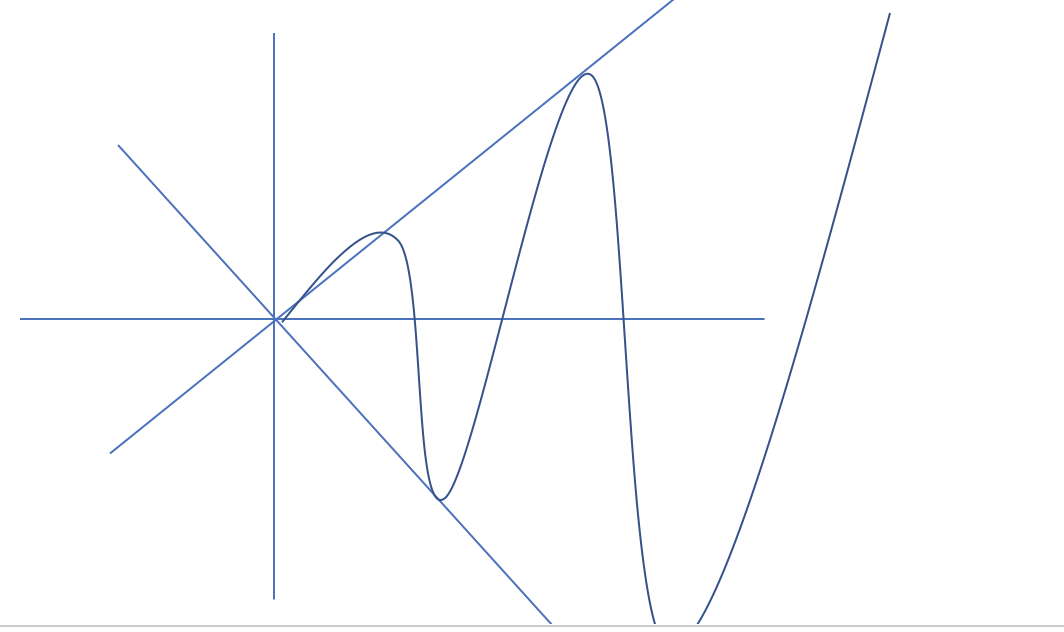
\includegraphics[width=8cm]{week7}
\end{figure}


\end{enumerate}
\begin{remark}
\begin{enumerate}
\item
Again, the model is suitable when $y$ is small as it's the maximum amplitude can only be the width of the bridge.
\item Why we separate into two case?\\
When $w=w_0$, the solution in first case doesn't hold.\\If we pick some part in first term of general solution $c_1\cos(w_0t)$ and let $w\rightarrow w_0$, we can see that
\[\frac{F_0}{m(w^2-w_0^2)}\cos wt-\frac{F_0}{m(w^2-w_0^2)}\cos w_0t=\frac{F_0}{m(w^2-w_0^2)}(\cos wt-\cos w_0t)
\]
By L'hospital's rule, it is equal to $-\frac{F_0}{2mw}t\sin wt\rightarrow -\frac{F_0}{2mw_0}t\sin w_0t$ which is equal to the specific solution of the equation in second case.
\end{enumerate}
\end{remark}
\begin{example}
\begin{figure}[H]
\centering
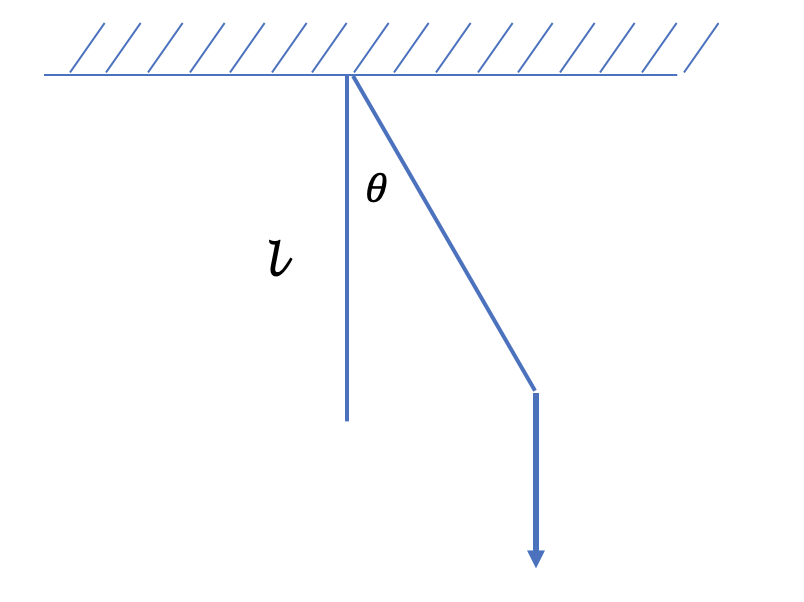
\includegraphics[width=8cm]{week7_taibei}
\end{figure}

The world largest damper is modelized as a pendulum with period 7sec. The aim is to find the length of the cable to hung the mass.\\
Because of energy conservation,
\[\frac{1}{2}ml^2(\frac{\diff \theta}{\diff t})^2+mgl(1-\cos\theta)\equiv constant
\]
Differentiate $\theta$,
\[ml^2\theta\pp\theta\p+mgl\theta\p\sin\theta=0
\]
\[\theta\pp+\frac{g}{l}\sin\theta=0
\]
\[\theta\pp+\frac{g}{l}\theta=0
\]
By physics, $w^2=\frac{g}{l}$, period=$2\pi\sqrt{\frac{l}{g}}=7$. We get l=12.18m.
\end{example}
\begin{example}
It is known that 1kg mass moves a spring $ \frac{49}{320}$m. If the mass is pulled down with an additional $\frac{1}{4}$m and released. Find amplitude, period, and frequency of the motion neglecting air resistance.
\[my\pp+cy\p+ky=0
\]
m=1kg, c=0,  $mg=k\Delta l~\Rightarrow$ $1kg\cdot9.8m/ sec^2=k\frac{49}{320}m$,  k=64
\[\left \{	\begin{gathered}
y\pp+64y=0\\
y(0)=\frac{1}{4}\\
y\p(0)=0.
\end{gathered}\right.
\]
\[y=c_1\cos(8t)+c_2\sin(8t)
\]
\[y(0)=c_1=\frac{1}{4}
\]
\[y\p(0)=0=-(\sin8t)8+8c_2\cos8t
\]
\[c_2=0
\]
\[y=\frac{1}{4}\cos(8t)
\]
Therefore, amplitude=0.25m and period=0.25$\pi$

\end{example}



